\chapter{Discussion}
Please tell more about conclusion and how to the next work of this study.

\section{hd Zulfikar Akram Nastuion / 1164081}
\subsection{Teori}
\begin{enumerate}
\item Jelaskan kenapa file suara harus di lakukan MFCC. dilengkapi dengan ilustrasi !
\par
MFCC (Mel Frequency Cepstrum Coefficients) merupakan metode untuk melakukan feature extraction, sebuah proses yang mengkonversikan sinyal suara menjadi beberapa parameter. Dimana dalam python MFCC digunakan untuk melakukan extraksi suara menjadi bentuk vektor. Mengapa perlu dilakukan ?, dikarenakan mesin tidak dapat membaca data selain bilangan biner dan vektor, maka dari itu untuk mempermudah pembacaan data oleh mesin perlu dilakukannya MFCC. Disini saya akan memberikan ilustrasi sederhana dimana ada sebuah Machine Learning yang ingin membaca data dalam bentuk gelombang suara. Machine Learning tidak akan bisa membaca data tersebut, Mengapa ?, karena data tersebut masih berbentuk gelombang suara, untuk memahami Machine Learning perlu data dalam bentuk vektor, maka gelombang suara tersebut akan diubah menjadi bentuk vektor.
\item Jelaskan konsep dasar neural network. Dilengkapi dengan ilustrasi atau gambar !
\par
Neural Network atau Jaringan Saraf dimana memiliki neuron dan pada tiap neuron akan saling terhubung pada lapisan - laposan berikutnya. Pada lapisan pertama dimana terjadinya proses menerima input sedangkan pada lapisan terakhir akan memberikan output. Neural Network akan mengadopsi mekanisme berpikir sebuah sistem atau aplikasi yang menyerupai otak manusia, baik dalam pemrosesan berbagai sinyal elemen yang diterima, toleransi kesalahan atau error, dan parallel processing. Untuk contoh figure dapat dilihat pada figure \ref{1164081_1}.
	\begin{figure}[!htbp]
		\centering{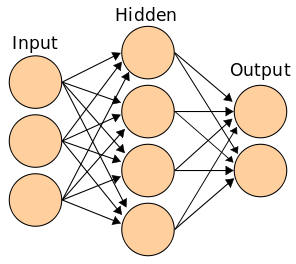
\includegraphics[scale=0.7]{figures/zulfikar/6/Teori/1164081_1.png}}
		\caption{Konsep Nural Network}
		\label{1164081_1}
	\end{figure}
\item Jelaskan konsep pembobotan dalam neural network. Dilengkapi dengan ilustrasi atau gambar !
\par
Dimana Bobot akan mewakili koneksi antar unit. Apabila bobot dari node 1 ke node 2 memiliki nilai yang kebih besar, hal ini menandakan bahwa neuron 1 memiliki pengaruh yang lebih besar terhadap neuron 2. Apabila nilai bobot mendekati nol hal ini menandakan akan merubah input namun tidak mengubah output dan apabila nilai bobot negatif hal ini menandakan akan meningkatkan input namun mengurangi output yang artinya bobot akan menentukan seberapa besar pengaruh input terhadap output. Untuk ilustrasi figure dapat dilihat pada figure \ref{1164081_2}.
	\begin{figure}[!htbp]
		\centering{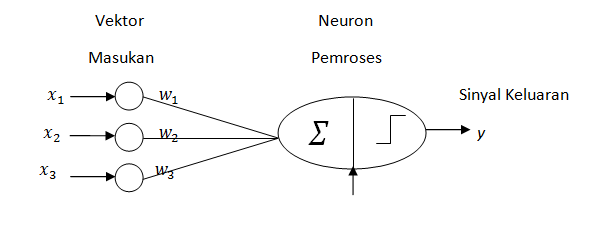
\includegraphics[scale=0.5]{figures/zulfikar/6/Teori/1164081_2.png}}
		\caption{Konsep Pembobotan}
		\label{1164081_2}
	\end{figure}	
\item Jelaskan konsep fungsi aktivasi dalam neural network. Dilengkapi dengan ilustrasi atau gambar !
\par
Dimana fungsi aktivasi ini merupakan operasi dalam matematika yang digunakan pada sinyal output y. Fungsi ini sering digunakan untuk mengaktifkan atau menonaktifkan neuron. Dimana perilaku dari neural network ini ditentukan oleh bobot dan input-output fungsi aktivasi yang telah ditetapkan. Contohnya dimana jaringan lapisan tunggal akan menkonversi nilai input dari suatu variabel yang bernilai continue ke suatu nilai output biner yaitu angka 0 dan 1. Untuk contoh figure dapat dilihat pada pada figure \ref{1164081_3}
	\begin{figure}[!htbp]
		\centering{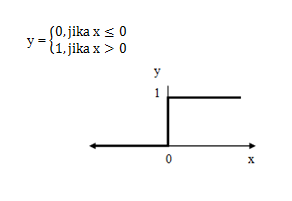
\includegraphics[scale=0.7]{figures/zulfikar/6/Teori/1164081_3.png}}
		\caption{Fungsi Aktivasi}
		\label{1164081_3}
	\end{figure}	
\item Jelaskan cara membaca hasil plot dari MFCC. Dilengkapi dengan ilustrasi atau gambar !
\par
Perhatikan figure \ref{1164081_4}, dimana terlihat bahwa warna biru merupakan suara terendah, mengapa ?, dikarenakan warna biru bernilai -300, sedangkan warna merah merupakah suara tertinggi dan bernilai 200. Jika diilustrasikan ada sebuah musik yang sedang dimainkan dan diperoleh datanya lalu diplot, maka akan terlihat seperti pada figure \ref{1164081_4}
	\begin{figure}[!htbp]
		\centering{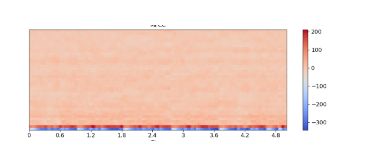
\includegraphics[scale=0.5]{figures/zulfikar/6/Teori/1164081_4.png}}
		\caption{Plot MFCC}
		\label{1164081_4}
	\end{figure}	
\item Jelaskan apa itu one-hot encoding. Dilengkapi dengan ilustrasi kode dan atau gambar !
\par
One-hot encoding merupakan representasi variabel berkategorikan sebagai vektor biner yang artinya hanya akang 0 dan 1. Dimana mengharuskan nilai categorinya berbentuk biner dan setiap nilai integer akan dipresentasikan kedalam vektor biner.  
\item Jelaskan apa fungsi dari np.unique dan to\_categorical dalam kode program . Dilengkapi dengan ilustrasi atau gambar !
\par
\begin{itemize}
\item Fungsi dari np.unique yaitu sebagai indeks array input yang memberikan nilai unik, sebagai indeks array unik yang merekonstruksi array input, dan menghitung berapa kali setiap nilai unik muncul dalam array input. 
\item Fungsi dari to\_categorical yaitu untuk mengubah vektor ke dalam matriks class biner.
\end{itemize}
\item Jelaskan apa fungsi dari Sequential dalam kode program. Dilengkapi dengan ilustrasi atau gambar !
\par
Dimana fungsi dari Sequential dalam source code program hanyalah sebagai tumpukan linear lapisan.
\end{enumerate}
